\documentclass{article}
\usepackage[fontsize=13pt]{fontsize}
\usepackage{geometry}
\usepackage{graphicx} % Required for inserting images
\usepackage[T2A]{fontenc}
\newgeometry{top=20mm, bottom=20mm, left=10mm, right=20mm}
\title{Дизайн документ}
\author{Пищаева Анастасия \\ Игонина Ксения \\ Иконников Андрей \\ Хохлов Тимофей \\ Аветисян Гаспар}
\date{Ноябрь 2024}

\begin{document}

\maketitle

\tableofcontents
\newpage

\section{Введение}
Этот документ содержит описание концепции и дизайна игры "Гномик в лесу", предназначенной для мобильных устройств. В нем описаны ключевые аспекты игры, включая геймплей, механики, мир, персонажей, а также технические детали разработки. Данный документ служит основой для дальнейшего планирования и реализации проекта.

\begin{itemize}
\item Комментарии по организации содержимого документа

Документ разделен на несколько основных разделов, каждый из которых описывает определенные аспекты игры:
\begin{itemize}

\item Введение - краткая формулировка всей идеи игры

\item Жанр и аудитория — сведения о целевой аудитории и жанре

\item Основные особенности игры — ключевые особенности и примерный объем игры

\item Описание игры — основная концепция

\item Предпосылки создания — "право на жизнь" для игры

\item Платформа — на чем планируется запуск игры
\end{itemize}

Дизайн-документ ориентирован на команду разработчиков и дизайнеров, а также на всех, кто будет участвовать в процессе создания игры.

\item Ссылки на использованные материалы, копирайты и прочее
\begin{itemize}


\item Концепт-арт и иконки: Все изображения, использованные в игре, были созданы дизайнером нашей команды.

\item Звуковые эффекты и музыка: Для разработки использована нелицензированная музыка.

\item Графика: Все использованные графические элементы являются оригинальными.
\end{itemize}

\item История изменений документа
\begin{center}
\begin{tabular}{| c | c | c | c |}
\hline
 Версия & Дата & Автор & Изменение \\  \hline
 1.0 & 2024-11-17 & Анастасия Пищаева & Написано 4 пункта введения для документа\\ \hline
 1.1 & 2024-11-17 & Игонина Ксения & Дописано введение и Концепт и Введение\\  \hline 
 1.2 & 2024-11-17 & Аветисян Гаспар & Написаны Жанр и аудитория и Основные особенности игры\\  \hline
 1.3 & 2024-11-17 & Хохлов Тимофей & Описание игры и Предпосылки создания\\  \hline
 1.4 & 2024-11-17 & Иконников Андрей & Системные требования\\ \hline 
 1.5 & 2024-11-27 & Хохлов Тимофей & Принципы игры\\  \hline
 1.6 & 2024-12-01 & Аветисян Гаспар & Персонаж игрока\\ \hline
 1.7 & 2024-12-01 & Анастасия Пищаева & Физическая модель\\ \hline
 1.8 & 2024-12-01 & Игонина Ксения & Элементы игры\\ \hline
 1.9 & 2024-12-01 & Иконников Андрей & Искусственный интеллект\\ \hline
 1.10 & 2024-11-27 & Хохлов Тимофей & Блок-схема\\  \hline
 1.11 & 2024-11-27 & Анастасия Пищаева & Функциональное описание и управление\\  \hline
 1.12 & 2024-12-01 & Аветисян Гаспар & Объекты интерфейса пользователя\\ \hline
 1.13 & 2024-11-17 & Игонина Ксения & Общее описание и Двумерная графика и анимация\\  \hline 


\end{tabular}
\end{center}

\item Список авторов
	\begin{itemize}
		\item Андрей Иконников — Главный разработчик.
		\item Тимофей Хохлов — Ответственный за программирование и техническую сторону проекта.
		\item Ксения Игонина — Ответственный за программирование и техническую сторону проекта.
		\item Анастасия Пищаева — Дизайнер.
		\item Гаспар Аветисян — Создатель музыкального сопровождения.
	\end{itemize}

\item Условные обозначения, сокращения и соглашения
	\begin{itemize}
            \item Гномик — Главный персонаж игры.
            \item Раннер — Тип игры, в которой игрок управляет персонажем, который автоматически движется вперед.
            \item UI — Пользовательский интерфейс.
            \item UX — Опыты пользователя.
	\end{itemize}

\item Другие сведения, необходимые для прочтения документа
	\begin{itemize}
            \item Для лучшего понимания дизайна игры рекомендуется ознакомиться с аналогичными играми жанра «раннер» на мобильных платформах, чтобы учитывать лучшие практики и выявить потенциальные улучшения.
            \item Раннер — Тип игры, в которой игрок управляет персонажем, который автоматически движется вперед.
            Дополнительные материалы, такие как концепт-арты и описание прототипа, могут быть предоставлены отдельно по запросу.
	\end{itemize}
\end{itemize}

\section{Концепция}

Этот документ описывает ключевые аспекты игры "Гномик в лесу", которая будет разработана как мобильный аркадный раннер с элементами платформера. Концепт-файл представляет собой обзор основных механик игры, целевой аудитории, особенностей и обоснования для её создания.

\subsection{Введение}

"Гномик в лесу" — это мобильная аркадная игра в жанре раннера, где игрок управляет маленьким гномом, который бежит через лес, избегая препятствий и собирая бонусы. Игра не имеет уровней, а её цель — пройти как можно дальше, увеличивая свой рекорд с каждым новым запуском. Лес всегда одинаков, но сложность игры возрастает с течением времени, предлагая игроку всё более сложные препятствия и вызовы. Игра ориентирована на детей и взрослых, обеспечивая простое управление и бесконечный игровой процесс.

\subsection{Жанр и аудитория}

\begin{itemize}
    \item \textbf{Жанр}: платформер с элементами приключения.
    \item \textbf{Возрастные ограничения}:
    \begin{itemize}
        \item \textit{7+}: сдержанный стиль с элементами фэнтези, не содержащий жестоких сцен.
    \end{itemize}
\end{itemize}

\subsection{Основные особенности игры}

\subsubsection{Ключевые особенности (USP)}
\begin{enumerate}
    \item \textbf{Интуитивно понятный геймплей:} простой и интуитивно понятный геймплей: Игра подходит для игроков всех возрастов благодаря простоте управления. Гномик автоматически бежит, а игроку нужно лишь уклоняться от препятствий и собирать бонусы с помощью свайпов или тапов.
    \item \textbf{Однородный фон:} в отличие от множества игр с меняющимися локациями, наш лес остаётся неизменным на протяжении всей игры. Это позволяет сосредоточиться на чистом и бесперебойном игровом процессе, где главной задачей становится преодоление все более сложных препятствий.
    \item \textbf{Бесконечный режим:} игра не имеет четкой финальной цели, и ее суть заключается в том, чтобы пройти как можно дальше. С каждым новым рекордом игрок сталкивается с более сложными препятствиями, но сам мир и фон остаются одинаковыми, что подчеркивает чисто аркадный и бесконечный характер игры.
    \item \textbf{Не требуется улучшение героя:} в отличие от многих игр, где игрок должен развивать персонажа и открывать новые способности, в нашей игре гномик остается неизменным. Это упрощает игру и делает её более доступной для быстрого старта и непрерывных сессий.
    \item \textbf{Фокус на рефлексах и внимании:} из-за того, что изменения в игровом процессе ограничены только увеличением сложности препятствий, игроку нужно опираться исключительно на свои рефлексы и концентрацию, что делает каждый момент на пути уникальным.
    \item \textbf{Уникальный саундтрек и звуковые эффекты:} Каждый игровой момент сопровождается атмосферной музыкой и звуками, создающими ощущение пребывания в волшебном лесу. Это добавляет игре особую атмосферу, несмотря на однообразие фона.
    \item \textbf{Доступность и легкость:} Игра не требует долгих сеансов и сложных решений. Она идеально подходит для коротких игровых сессий, что делает её отличным выбором для игры на ходу.
\end{enumerate}

\subsubsection{Примерный объем игры}
\begin{itemize}
    \item \textbf{Время прохождения:} из-за бесконечного игрового процесса с возможностью достижения рекордов, игра предоставляет игрокам практически неограниченное количество сессий. Среднее время одного игрового сеанса — 5-10 минут, но в зависимости от умения игрока, каждый новый запуск может длиться дольше.
\end{itemize}




\subsection{Описание игры}

Игрок управляет маленьким гномом, который стремится добраться домой через волшебный лес, наполненный препятствиями и опасностями. Он движется вперед-назад, и задача игрока — избегать встречающихся на пути ям, деревьев, рек и врагов, таких как лесные звери. Для этого нужно вовремя прыгать, уклоняться и кидаться маленькими звёздами. По ходу игры на пути гномика будут встречаться большие золотые звёзды, которые увеличивают количество набранных очков.

\noindentКаждый уровень сделан и отредактирован вручную, что исключает проблемы с невозможностью прохождения. Сложность возрастает с каждым пройденным этапом — появляются новые типы врагов и препятствий, а также становится сложнее собирать звёзды и набирать очки.

\subsection{Предпосылки создания}

\begin{itemize}
\item Общие тенденции рынка:
	\begin{itemize}
            \item Рост популярности инди-игр: 2D платформеры остаются востребованным жанром благодаря их доступности, ностальгическому стилю и возможности реализовать оригинальные идеи при относительно небольших ресурсах.
            \item Ностальгия и ретро-стиль: механики платформеров вызывают ностальгию у игроков, что способствует их популярности.
            \item Мобильные и казуальные игры: платформеры хорошо адаптируются для мобильных устройств и пользуются успехом у широкой аудитории.
	\end{itemize}

\item Обоснование «права на жизнь»:
	\begin{itemize}
            \item Учебный проект: Игра создается как учебный проект, что оправдывает её экспериментальный и образовательный характер. Это позволяет разработчикам на практике изучить полный цикл разработки.
            \item Ориентация на малые ресурсы: 2D платформеры требуют меньше технических и временных затрат, что делает их идеальным выбором для студентов.
            \item Привлекательность для широкой аудитории: Простая механика и доступный игровой процесс способны заинтересовать как детей, так и взрослых.
            \item Возможность реализации уникальных идей: Платформеры предоставляют широкие возможности для экспериментов с дизайном уровней, механиками и художественным стилем.
	\end{itemize}
\end{itemize}


\subsection{Платформа}
    \item Системные требования:
    	\begin{table}[h]
        \centering
        \begin{tabular}{|c|c|c|}
            \hline
            Требования & Минимальные & Рекомендуемые \\
            \hline
            Операционная система & Windows 7 x64, Mac OS 10.15.1 & Windows 10 x86, OS X 'Big Sur'\\
            \hline
            Процессор & CPU с тактовой частотой 2.4Ghz& CPU с тактовой частотой 3.0Ghz \\
            \hline
            ОЗУ & 1024МБ & 2048МБ \\
            \hline
            CD-ROM привод & зачем ? & зачем ? \\
            \hline
            Свободное место на HDD & 30МБ & 100МБ \\
            \hline
            Видеоадаптер & Любой с поддержкой DX10 & Любой с поддержкой DX10 \\
            \hline
            Звуковая Карта & Relatek ALC1220 & Relatek ALC1220 \\
            \hline
            Управления & Клавиатура и геймпад & Клавиатура и геймпад \\
            \hline
        \end{tabular}
        \caption{Таблица с системными требованиями}
        \label{tab:systemrequirements}
\end{table}


\section{Функциональная спецификация}

Этот пункт содержит основное описание игры с точки зрения игрока. Именно здесь раскрываются все возможности игры, что поможет сложит представление об игре перед её непосредственным запуском. Речь идёт именно о геймплее, без обширного описания технических деталей и выкладок с точки зрения разработчика. 


\subsection{Принципы игры}

В принципах игры описано всё то, что игрок будет видеть и ощущать по ходу прохождения. Игровой процес полностью расписан: от сюжета до важных для получения полного игрового экспириенса тонкостей.


\subsubsection{Суть игрового процесса}

Суть игрового процесса игры \textbf{<<Гномик в лесу>>} заключается в управлении персонажем, преодолении препятствий и собиранием звёз для набора очков. Игроку необходимо вовремя реагировать на различные препятствия и угрозы, чтобы пройти как можно дальше, собирая бонусы и избегая поражения.

Главный герой --- гномик Грек --- стремится преодолеть волшебный лес, используя свои навыки ловкости и реакции. Игровой процесс сосредоточен на последовательном преодолении препятствий, таких как ямы, деревья и враги, путём выполнения следующих действий:
\begin{itemize}
    \item \textbf{Прыжки и уклонения}: Игрок управляет гномиком с клавиатуры или геймпада, преодолевая препятствия и проходя уровни.
    \item \textbf{Взаимодействие с врагами}: Враги требуют активных действий. Игрок должен уклоняться от пчёл или поражать ящериц метанием маленьких звёздочек.
    \item \textbf{Сбор предметов}: Золотые звёзды расположены на уровне так, чтобы мотивировать игрока рисковать и тщательно планировать свои движения.
\end{itemize}

\paragraph{Основные особенности игрового процесса:}
\begin{enumerate}
    \item \textbf{Постоянное нарастание сложности}: С каждым этапом сложность возрастает за счёт  усложнения препятствий и появления новых врагов.
    \item \textbf{Фокус на рефлексах и внимании}: Игра проверяет быстроту реакции и способность планировать действия на ходу.
    \item \textbf{Простота управления}: Простой интерфейс и отзывчивое управление делают игру доступной для игроков любого возраста.
\end{enumerate}

\noindent <<Гномик в лесу>> предлагает игрокам испытание на выносливость и внимательность, а также захватывающий опыт в погружении в сказочный лес. Игроки стремятся к новым рекордам, одновременно наслаждаясь простотой механик и атмосферой игры.


\subsubsection{Ход игры и сюжет}

\textbf{Типичный сеанс игры:}
\begin{enumerate}
    \item \textbf{Главное меню:} Игрок меняет разрешение экрана под своё устроймтво, выбирает уровень или может начать с первого, нажав новая игра.
    \item \textbf{На 1 уровне:} Лес выглядит спокойным, препятствия просты для преодоления — игрок втягивается в игровой процесс. Уровень предназначен для знакомства с управлением и получения общего понимания игровых механик.
    \item \textbf{Рост сложности:} С каждым последующим уровнем растёт сложность прохождения:
    \begin{itemize}
        \item Появление движущихся платформ и падающих препятствий.
        \item Враги (осы и ящерицы), которые нападают на игрока, как только начинают его видеть. Пройти мимо не получится, их обязательно нужно победить. Сталкновение с ними вернёт игрока на начало уровня.
        \item Набор очков становится всё труднее из-за сложного расположения звёздочек.
    \end{itemize}
    \item \textbf{На 5 Уровене:} Кульминация игры и самый сложный для прохождения уровень. Содержит все неприятности прошлых уровней, но в большем количестве.
\end{enumerate}

\noindent\textbf{Сюжет:} 

Далеко-далеко, в самом сердце волшебного леса, живет маленький гномик по имени Грек. Однажды, прогуливаясь по лесу, он слишком далеко забрел и потерял путь домой. Теперь ему предстоит пройти через лес, полный различных препятствий, чтобы вернуться в свой уютный домик.

Лес полон загадок: здесь растут высокие деревья, через которые нужно пробираться, а узкие тропинки часто скрыты за густым кустарником. Но лес — не только мир красоты. На пути Грека подстерегают два опасных врага: хитрые ящерицы, которые прячутся среди камней и могут напасть, если он не будет осторожен, и опасные пчелы, которые живут в лесных ульях и могут устроить настоящее нападение, если их потревожить.

Греку нужно быть быстрым и внимательным, чтобы избежать этих врагов и преодолеть все препятствия, которые встретятся на пути. Лишь тот, кто сможет ловко прыгать через камни, перепрыгивать через ямы и обходить врагов, сможет достичь своей цели и вернуться домой.

Помоги Греку пройти через лес, обойдя все ловушки и избегая ящериц и пчел! Только самый решительный и ловкий гномик сможет пройти этот путь до конца!

\subsection{Физическая модель}
В этой игре физическая модель ориентирована на взаимодействие персонажа — маленького гномика — с окружающим миром, включая препятствия, врагов и объекты на пути. Основной акцент сделан на реалистичности движения, взаимодействий с объектами и точности реакции на действия игрока. Вся физика движений и действий должна быть достаточно интуитивно понятной, но при этом достаточно глубокой для создания ощущения динамики и вовлеченности.

\begin{enumerate}
  \item \textbf{Перемещения:} 
    \begin{itemize}
      \item \textbf{Гномик:} Персонаж перемещается по двумерному игровому миру влево и вправо, а также прыгает, уклоняется и использует звезды для атаки врагов.
      \begin{itemize}
        \item Горизонтальное движение: Используется стандартное линейное перемещение по оси X с плавной инерцией. При отпускании клавиши или кнопки движения скорость уменьшается согласно законам физики.
            \item Прыжки: Гномик может прыгать на определенную высоту. Во время прыжка он также может перемщаться влево или вправо, для чего используется стандартная парабола движения, учитывающая гравитацию. Прыжок может быть с разной амплитудой в зависимости от того, насколько долго игрок удерживает кнопку.
            \item Касание земли: При касании гномика с землей (или любым объектом, который он может пройти, например, бревнами) происходит мягкое приземление на объект.
            \item Столкновения с препятствиями: В случае столкновения с объектом (например, деревом или землей), гномик останавливается.
      \end{itemize}
      \item \textbf{Оса:} Оса летает в воздухе и будет следовать за гномиком, пока тот не уничтожит её с помощью звезд. Если гномик меняет направление или прыгает, оса будет точно следовать за ним, поддерживая траекторию полета с учётом движения персонажа.
      \begin{itemize}
        \item Механика движения:
Оса использует линейное следование за гномиком. При этом её скорость может быть настроена в зависимости от типа сложности, чтобы она не отставала.
При преследовании оса будет корректировать своё положение в пространстве, используя векторную скорость: каждый раз, когда гномик меняет позицию (двигаясь влево или вправо, или прыгая), оса будет немедленно перенастраивать свой путь, чтобы оставаться на его траектории. 
        \item Движение по вертикали: Если гномик меняет вертикальное положение (прыжок), оса также будет корректировать своё вертикальное положение, чтобы следовать за ним по той же высоте. Это заставляет её лететь «по зафиксированным координатам», пока не столкнется с гномиком или не будет уничтожена.
При ударе звездой или попадании в другого врага, оса уничтожается, что прерывает её движение.
      \end{itemize}
      \item \textbf{Ящерица:} Ящерица не двигается, пока не окажется в зоне видимости гномика. Как только гномик входит в её поле зрения, ящерица начинает двигаться в его направлении.
      \begin{itemize}
        \item Направление движения: Ящерица движется к гномику, но в отличие от осы, её движение по прямой и зависит от того, где находится гномик. Если гномик меняет направление, ящерица также меняет свою траекторию, но с некоторой задержкой. Это имитирует реакцию на изменения в движении гномика.
        \item Скорость: Ящерица будет двигаться с фиксированной скоростью, которая может быть изменена в зависимости от уровня сложности игры. Если гномик сбегает или перемещается слишком быстро, ящерица может замедлить свой преследующий темп, чтобы создать сложность.
        \item Логика уклонений: Если гномик уклоняется или прыгает, ящерица также будет пытаться изменить направление, чтобы не упустить цель. 
      \end{itemize}
    \end{itemize}
  \item \textbf{Боевые действия:}
  \begin{itemize}
    \item \textbf{Звезды:} Гномик использует маленькие звезды как оружие для защиты от врагов. Звезды движутся по траектории, которая рассчитывается как линия с постоянной начальной скоростью и углом наклона (угол определяется направлением, в котором был выпущен снаряд).
    \begin{itemize}

        \item Скорость звезды: Звезда двигается с постоянной скоростью по траектории, пока не столкнется с объектом (например, с врагом). При столкновении с врагом происходит моментальный эффект (например, урон или исчезновение врага).
    \end{itemize}
  \end{itemize}
  \item \textbf{Общие формулы и физика:}
  \begin{itemize}
    \item \textbf{Гравитация:} Все объекты в игре подвержены влиянию гравитации, что влияет на падение и движение гномика. Стандартная сила притяжения на уровне 9.8 м/с² применяется к объектам.
    \item \textbf{Скорость и ускорение:}
    \begin{itemize}
      \item Для движения по земле скорость фиксированная.
      \item Прыжок имеет начальную скорость, которая равна произведению силы на массу персонажа, с учетом сопротивления воздуха.
    \end{itemize}
    \item \textbf{Столкновения:} Когда гномик сталкивается с объектом (деревом, землей), рассчитывается момент силы столкновения, который влияет на его скорость, и происходит "отскок" или замедление (остановка). В случае с врагами или ловушками (вода), при столкновении с ними гномик исчезает.
    
  \end{itemize}  
\end{enumerate}

\subsection{Персонаж игрока}

\subsubsection{Имя} 
Грек

\subsubsection{Внешность} 
Грек — маленький гномик с яркими рыжими волосами, которые подчеркивают его энергичность и решительность. Его большие, выразительные жёлтые глаза отражают искреннее любопытство и смелость. Грек одет в оранжево-коричневую одежду с золотистыми элементами, символизирующую тепло и связь с природой. На спине у него удобный рюкзак, в котором он хранит всё необходимое для путешествий по лесу.

\subsubsection{Характер и личность} 
Грек — дружелюбный, любознательный и решительный персонаж, который никогда не боится трудностей. Он заботится о природе и стремится защищать её от любых угроз. Несмотря на свой небольшой рост, Грек обладает большим сердцем и уверенностью в себе, что помогает ему справляться даже с самыми сложными ситуациями.

\subsubsection{Характеристики и способности} 
\begin{itemize}
    \item \textbf{Сила:} Средняя. Грек может нести лёгкие предметы и активно взаимодействовать с окружением.
    \item \textbf{Ловкость:} Высокая. Он умело перепрыгивает через препятствия, избегает ловушек и быстро реагирует на опасности.
    \item \textbf{Интеллект:} Выше среднего. Грек разгадывает загадки леса и использует свой ум для обхода врагов.
    \item \textbf{Выносливость:} Хорошая. Он готов к долгим путешествиям и сражениям с лесными угрозами.
\end{itemize}

\subsubsection{Роль в игровом мире} 
Грек — искатель приключений, который оказался далеко от своего уютного домика. Его цель — найти дорогу домой, преодолев опасности и загадки волшебного леса. Он становится надёжным союзником для природы, сражаясь с врагами, такими как хитрые ящерицы и опасные пчёлы.

\subsubsection{Особенности} 
\begin{itemize}
    \item Умение находить бонусные предметы.
    \item Быстрое освоение новых навыков, таких как акробатические прыжки, кидание звезд, сбор бонусных предметов.
\end{itemize}

\subsubsection{Сюжетная роль} 
История Грека — это путь о возвращении домой через полный загадок лес, где каждое препятствие — это проверка его навыков и решимости. Он вдохновляет игрока верить в свои силы и находить выход даже в самых сложных ситуациях.



\subsection{Элементы игры}

\subsubsection{Юниты и строения (RTS, TBS)}
В данном контексте эти элементы не применимы, так как игра не относится к жанрам RTS (реального времени стратегий) или TBS (пошаговых стратегий). В игре нет юнитов или строений, которые бы строились или управлялись в процессе.

\subsubsection{Предметы (Items)}
\textbf{Золотые звезды:} Главный сборный элемент игры. Звезды увеличивают очки игрока, а их сбор стимулирует активные и рисковые действия. Эти предметы расположены в разных частях уровня, что заставляет игрока проявлять ловкость и стратегию в выборе пути.
\begin{itemize}
    \item \textbf{Особенности:} Звезды увеличивают количество очков, их количество и расположение варьируются в зависимости от сложности.
    \item \textbf{Влияние на игрока:} Мотивирует к сбору, предоставляет дополнительные очки, создаёт элемент соревнования (самый высокий счёт).
\end{itemize}

\subsubsection{Оружие (FPS, RPG)}
Так как "Гномик в лесу" не является шутером или ролевой игрой, оружия у игрока нет.

\subsubsection{NPC и персонажи}
\begin{itemize}
    \item \textbf{Гномик Грек:} Главный персонаж игры. Игрок управляет им, преодолевая препятствия и собирая бонусы.
    \begin{itemize}
        \item \textbf{Особенности:} Не имеет способности улучшаться или изменяться в процессе игры. Его поведение стабильно: он всегда движется вперед, может прыгать и уклоняться.
    \end{itemize}
    \item \textbf{Враги:} Пчёлы и ящерицы, с которыми Гномик сталкивается на пути.
    \begin{itemize}
        \item \textbf{Особенности:} Враги требуют действий игрока — уклонение или прыжки.
        \item \textbf{Влияние на игрока:} Эти враги создают дополнительные сложности в процессе игры, заставляя игрока быть внимательным и реагировать на угрозы.
    \end{itemize}
\end{itemize}

\subsubsection{Транспортные средства (Simulators)}
В игре нет транспортных средств, так как она является платформером с элементами раннера. Персонаж (Гномик) движется самостоятельно без необходимости использования транспортных средств.

\subsubsection{Карты}
Игра происходит в одном лесу, который является единственным уровнем на протяжении всей игры. Сложность игры постепенно увеличивается по мере того, как игрок продвигается, что создаёт ощущение прогресса.
\begin{itemize}
    \item \textbf{Особенности карты:} Лес — это статичный фон, но с увеличением сложности появляется больше препятствий и врагов.
    \item \textbf{Влияние на игрока:} Из-за однообразия карты фокус игры смещается на преодоление препятствий и накопление очков, а не на изменение окружающей среды.
\end{itemize}

\subsubsection{Прочее}
\begin{itemize}
    \item \textbf{Система очков:} Система очков позволяет игроку оценивать свой прогресс. Каждое препятствие, которое преодолено, приносит очки.
    \begin{itemize}
        \item \textbf{Особенности:} Очки играют роль мотивации для игроков. Наибольшее количество очков становится рекордом, с которым игрок может соревноваться.
        \item \textbf{Влияние на игрока:} Мотивирует к повторным играм и улучшению результатов.
    \end{itemize}
\end{itemize}

\subsection{Искусственный интеллект}
ИИ используется для разнообразия игрового процесса. Так, ИИ наделены только противники - Ящерица и Оса. Каждый из противников использует свою, уникальную стратигею, для того. чтобы отправить игрока в начало уровня.
\subsubsection{Ящерица}
Ящерица - самый простой и очевидный противник в игре, при этом не снижающией темпа самой игры. Данный противник перемещается довольно быстро, следуя за главным героем, пока не настигнет его, тем самым требуя от игрока высокой скорости реакции на происходящее на экране.
\subsubsection{Оса}
Оса - достоинный соперник. Она нападает с воздуха, пикируя на главного героя. Такой противник вызывает сложности у игрока, который не обуздал с полной мере управление игры.


\subsection{Графика и видео}

\begin{itemize}
    \item Общее описание
    \begin{itemize}
        \item Техническое исполнение:
        Игра использует 2D-графику. Все игровые сцены, персонажи, анимации и объекты будут представлены в двумерной плоскости с разнообразными визуальными эффектами, которые усиливают атмосферу.
        \item Стилистика, атмосфера и палитра:
        Визуальный стиль игры ориентирован на минимализм и четкость, с акцентом на плавные анимации и выразительные элементы интерфейса. В дизайне используются приглушенные пастельные тона для создания расслабляющей и атмосферной обстановки, с контрастными акцентами, подчеркивающими важные элементы игрового процесса, например, самого игрока. Важной особенностью является использование ретро-пиксельной графики, которая создает чувство ностальгии, но с современными визуальными эффектами для усиления динамичности.
        
        Атмосфера игры определяется через меланхоличные пейзажи и внимание к мелким деталям, что позволяет погружать игрока в уникальный мир игры. Все визуальные элементы — от фона до персонажей — имеют согласованную цветовую палитру, что помогает создать ощущение глубины и пространства в двумерном мире. Цвета используются для акцентирования внимания на ключевых элементах, таких как объекты взаимодействия, враги и достижения, поддерживая эмоциональный отклик игрока в каждом моменте игры.
        \item Другие общие сведения:
        Графика будет оптимизирована для работы на различных устройствах, обеспечивая плавную работу на мобильных платформах и ПК. Для улучшения взаимодействия с пользователем будет использована интуитивно понятная интерфейсная графика, поддерживающая различные разрешения экранов. 
    \end{itemize}

    \item Двумерная графика и анимация
    \begin{itemize}
        \item Интерфейс:
        Интерфейс будет включать в себя все основные элементы, необходимые для взаимодействия с игроком: количество звезд, меню. Дизайн интерфейса будет минималистичным и в то же время информативным, с четким выделением активных элементов, что позволит игроку легко ориентироваться в игре.
        \item Эффекты:
        Весь визуальный стиль сосредоточен на чистоте и простоте изображения, без добавления сложных анимаций. Все взаимодействия и изменения в игре будут переданы через изменения в анимированных персонажах и их поведении, а также через различные визуальные особенности фона и объектов, создающих атмосферу мира игры.
        \item Персонажи, строения и юниты:
        Все персонажи игры выполнены в 2D с четко прорисованными деталями. Каждый персонаж (главный герой) имеет уникальные анимации для движений, атак и взаимодействий с игровым миром. Все персонажи и юниты будут отображаться через простые, но выразительные анимации, что придает динамичность игровому процессу.
        \item Игровой мир (ландшафты и статические объекты):
        Лес и холма служит фоном для всей игры и создаёт атмосферу спокойствия и уединенности. Ландшафт выполнен в стиле самой игры с плавными переходами цветов и деталей, выполненными с помощью явления параллакса. Изображение леса нестатично, с изменениями в течение игры.
        
        Фон леса выполняет роль основного окружения, и взаимодействие с ним ограничивается движением персонажа. Все элементы фона, такие как холма и небо, являются частью визуальной среды, которая задает тон и атмосферу игры.
    \end{itemize}
\end{itemize}


\subsection{Интерфейс пользователя}
В этом разделе будет описан весь UI, который игрок сможет увидеть в игре.

\subsubsection{Блок-схема}
Ниже приведино описание всех функций гланого меню, которое грок видет каждый раз при входе в игру, в виде блок-схемы

\begin{figure}[h]
    \center{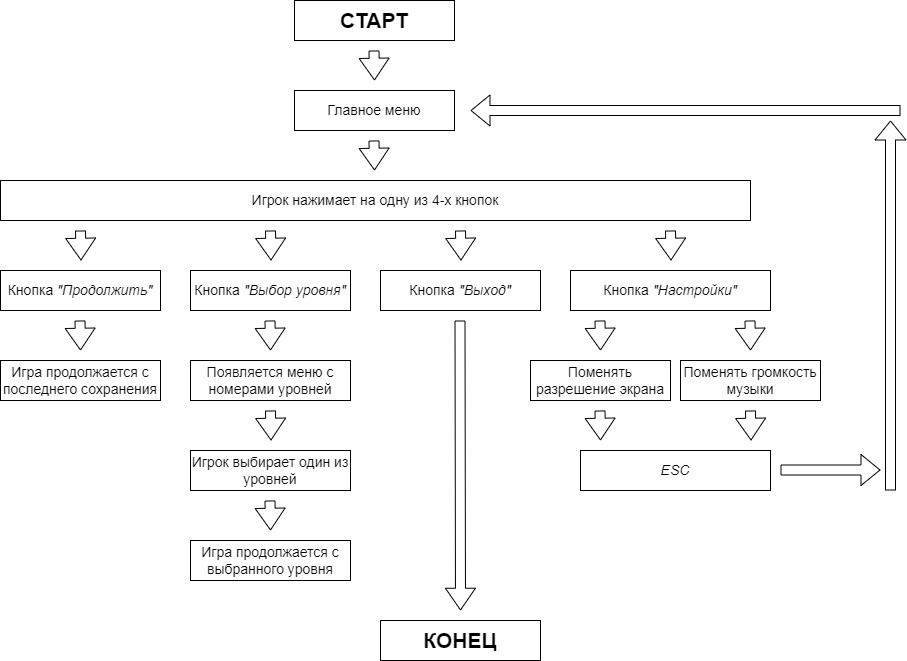
\includegraphics[width=1\linewidth]{Main_menu}}
    \caption{Возможное взаимодействие игрока с главным меню}
    \label{ris:image}
\end{figure}

\subsection{Интерфейс пользователя}
\subsubsection{Блок-схема}
\subsubsection{Функциональное описание и управление}
\begin{enumerate}
	\item \textbf{Старт} 
	Пользователь запускает приложение, которое переходит на Главное меню.
	\item \textbf{Главное меню} В главном меню отображаются четыре кнопки, каждая из которых выполняет определенное действие:
	\begin{itemize}
		\item \textbf{Кнопка "Продолжить"}
		\begin{itemize}
			\item Возобновляет игру с последнего сохранения.
			\item Пользователь возвращается к текущему прогрессу.
		\end{itemize}
		\item \textbf{Кнопка "Выбор уровня"}
		\begin{itemize}
			\item Открывается меню выбора уровня, где отображается список доступных уровней.
			\item Пользователь выбирает уровень из списка, после чего игра продолжается с указанного уровня.
		\end{itemize}
		\item \textbf{Кнопка "Настройки"}
		\begin{itemize}
			\item Открывается меню настройки, где доступны следующие параметры:
			\begin{itemize}
				\item Изменение разрешения экрана — позволяет настроить качество и разрешение изображения.
				\item Изменение громкости музыки — регулирует громкость фонового музыкального сопровождения и отключить функциональные звуки (стрельба/прыжки)
			\end{itemize}
			\item Выход из меню настроек осуществляется нажатием клавиши ESC.
		\end{itemize}
		\item \textbf{Кнопка "Выход"}
		Завершает работу приложения.
	\end{itemize}
	\item \textbf{Игровой процесс}
	Игра происходит в формате отдельных уровней, где игрок может свободно передвигаться, взаимодействовать с объектами и выполнять различные действия. Основные аспекты игрового процесса:
	\begin{itemize}
		\item \textbf{Перемещение персонажа:}
		\begin{itemize}
			\item A / Стрелка "влево" — движение влево.
			\item D / Стрелка "вправо" — движение вправо.
			\item Space — прыжок.
		\end{itemize}
		\item \textbf{Атака:}
		\begin{itemize}
			\item Левая кнопка мыши — атака.
		\end{itemize}
		\item \textbf{Меню паузы:}
		\begin{itemize}
			\item ESC — вызов меню паузы для настройки параметров игры или выхода в главное меню.
		\end{itemize}
	\end{itemize}
	\item \textbf{Общая структура управления}
	\begin{itemize}
		\item Перемещение и действия интуитивны, поддерживаются как стандартные клавиши для ПК, так и для геймпадов.
		\item Игровой мир позволяет пользователю исследовать локации и взаимодействовать с окружением.
		\item Возврат в главное меню или настройки доступен в любой момент через меню паузы (клавиша ESC).
	\end{itemize}
\end{enumerate}


\clearpage % переход на новую страницу

\subsection{Объекты интерфейса пользователя}

\subsubsection{Игровой интерфейс}
\begin{itemize}
    \item \textbf{Стандартные элементы:}
    \begin{itemize}
        \item \textbf{Счетчик звезд:} Показывает текущее количество собранных звезд. Расположен в верхнем левом углу экрана.
    \end{itemize}
    \item \textbf{Нестандартные элементы:}
    \begin{itemize}
        \item \textbf{Игровой персонаж:} Гномик, управляемый игроком. Может перемещаться влево/вправо, прыгать и взаимодействовать с объектами.
        \item \textbf{Объекты взаимодействия:}
        \begin{itemize}
            \item Звезды: Элементы коллекционирования. Увеличивают общий счет игрока.
            \item Враги (столкновение с ними вернёт игрока на начало уровня):
            \begin{itemize}
                \item \textbf{Кусты с шипами:} наносят сильный урон при контакте.
                \item \textbf{Ящерицы:} двигаются и атакуют при приближении.
                \item \textbf{Пчёлы:} могут атаковать с воздуха.
            \end{itemize}
	    \item Препятствия:
            \begin{itemize}
                \item \textbf{Камни:} блокируют путь игрока.
                \item \textbf{Ямы:} падение в них приводит к потере прогресса.
            \end{itemize}
        \end{itemize}
        \item \textbf{Игровая среда:}
        \begin{itemize}
            \item Платформы: основные поверхности для передвижения игрока.
            \item Вода: падение в воду приводит к фатальному иходу.
        \end{itemize}
        \item \textbf{Фон:} статический задний план, создающий атмосферу волшебного леса.
    \end{itemize}
\end{itemize}

\subsubsection{Главное меню}
\begin{itemize}
    \item \textbf{Стандартные элементы:}
    \begin{itemize}
        \item Кнопки:
        \begin{itemize}
            \item \textbf{Продолжить:} возвращает игрока к текущей игровой сессии.
            \item \textbf{Выбор уровня:} открывает меню выбора одного из пяти уровней.
            \item \textbf{Настройки:} переход в меню настройки параметров игры.
            \item \textbf{Выход:} завершение игровой сессии и выход из приложения.
        \end{itemize}
    \end{itemize}
    \item \textbf{Нестандартные элементы:}
    \begin{itemize}
        \item Фон: лесная сцена с деревьями и кустарниками.
    \end{itemize}
\end{itemize}

\subsubsection{Меню выбора уровня}
\begin{itemize}
    \item \textbf{Стандартные элементы:}
    \begin{itemize}
        \item Список уровней: игрок может выбрать один из пяти доступных уровней.
    \end{itemize}
    \item \textbf{Нестандартные элементы:}
    \begin{itemize}
        \item Каждый уровень отличается уникальными врагами:
        \begin{itemize}
            \item \textbf{3 и 5 уровни:} Враги — ящерицы.
            \item \textbf{4 уровень:} Враги — пчёлы.
        \end{itemize}
    \end{itemize}
\end{itemize}


\end{document}
